\documentclass[a4paper,12pt]{article}

% --- 必要パッケージ ---
\usepackage{amsmath,amssymb}
\usepackage{geometry}
\usepackage{graphicx}
\usepackage{hyperref}
\usepackage{float}
\usepackage{fontspec}
\usepackage{xeCJK}
\usepackage{caption}
\usepackage{subcaption} % 副図のために追加
\usepackage{url}
\usepackage{tabularx}
\usepackage{booktabs}
\usepackage{enumitem}

% --- 日本語フォント設定 ---
\setmainfont{Noto Serif CJK JP}
\setCJKmainfont{Noto Serif CJK JP}

% --- ページ設定 ---
\geometry{margin=1in}

% --- ハイパーリンク設定 ---
\hypersetup{
    colorlinks=true,
    linkcolor=blue,
    citecolor=blue,
    urlcolor=blue
}

% --- 図キャプション設定 ---
\captionsetup{format=plain,labelsep=period,justification=centering,font={small,sf}}


% ===== ドキュメント開始 =====
\begin{document}

\title{Supplementary Information for \\ ``Observational Evidence for a Cosmic Quadrupole Anisotropy: ...''}
\author{Hiroto~Iwasaki}
\date{\today}
\maketitle

\section*{S1. \#1点構造の頑健性評価の詳細}
\label{sec:supp_robustness}

本補足資料では、論文E本体の§2で要約された\#1点構造の頑健性評価について、その詳細な手法と結果を記述する。

\subsection*{S1.1. 幾何学的構造の再現性:t-SNEによる検証}
\label{subsec:supp_geometry}

論文CでUMAPを用いて発見された、準励起点のクラスター形成と\#1点の空間的相関という幾何学的構造が、特定の次元削減アルゴリズムのアーティファクトではないことを確認するため、異なる非線形次元削減手法であるt-SNE (t-distributed Stochastic Neighbor Embedding) を用いて再解析を行った。

解析対象の4次元特徴空間(情報ポテンシャル、零点間隔、$\kappa(p)$、対数化素数)をt-SNEで2次元に投影した結果を、図\ref{fig:supp_tsne_projection}に示す。

\begin{figure}[H]
    \centering
    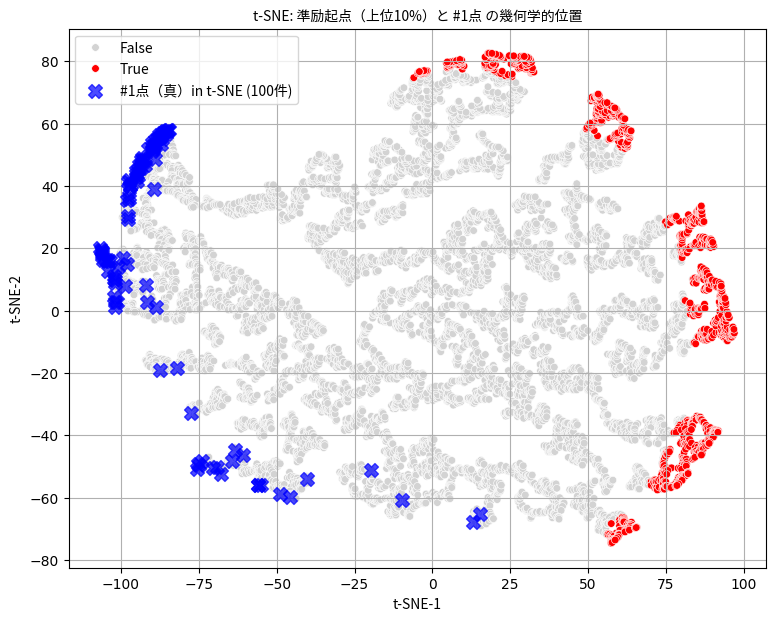
\includegraphics[width=0.8\linewidth]{S1_tsne_projection_robustness.png}
    \caption{t-SNEによる2次元投影結果。赤点は準励起点、青いXマーカーは\#1点を示す。準励起点が明確なクラスターを形成し、\#1点がそのクラスターの内部または近傍に局在する傾向が明瞭に観測され、これはUMAPによる結果と定性的に一致する。}
    \label{fig:supp_tsne_projection}
\end{figure}

図\ref{fig:supp_tsne_projection}が示すように、準励起点(赤点)はランダムに分布せず、複数のクラスターを形成している。さらに、\#1点(青いXマーカー)の多くは、これらの準励起点クラスターと強く相関した位置に存在する。この主要な幾何学的特徴がUMAPとt-SNEの両方で一貫して観測されたことは、この構造がデータに内在する本質的なものであることの強力な証拠となる。

\subsection*{S1.2. 動的同期の普遍性:複数領域でのFFT解析}
\label{subsec:supp_fft}

次に、t-SNE空間(図\ref{fig:supp_tsne_projection})上で特定された、準励起点および\#1点が特徴的な分布を示す4つの候補領域(候補領域①~④)からデータシーケンスを抽出し、指標間の動的同期が普遍的な特徴であるかを検証した。各シーケンスは、対応する情報ポテンシャルの値で昇順にソートした上でFFT解析を行った。

図\ref{fig:supp_fft_regions}に、4つの各候補領域における三指標(情報ポテンシャル、$\mathrm{d}c/\mathrm{d}t$、$\kappa(p)$)のFFTスペクトルを示す。また、各解析から得られた卓越周波数と位相の値を、表\ref{tab:supp_fft_peak_results}にまとめる。

\begin{figure}[H]
    \centering
    \begin{subfigure}{0.48\linewidth}
        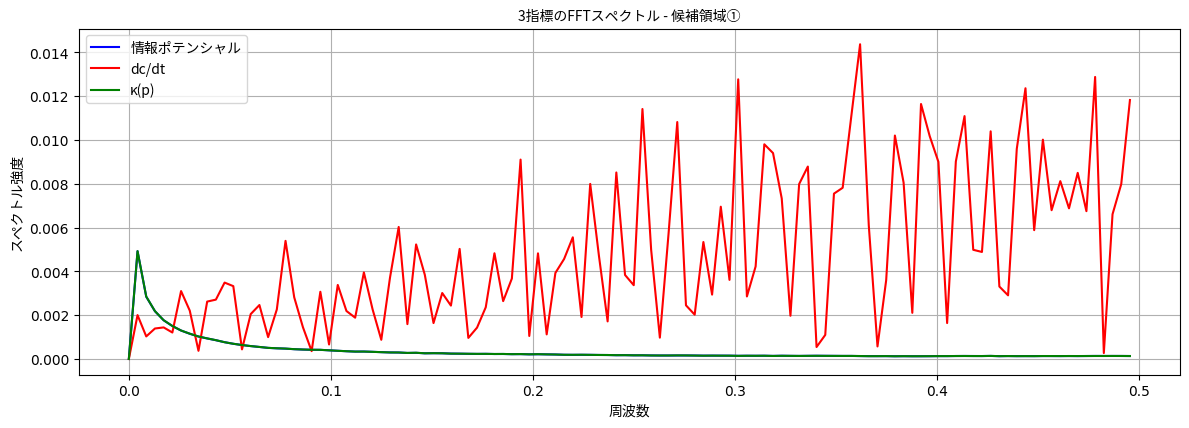
\includegraphics[width=\linewidth]{S1_fft_spectre_seq1.png}
        \caption{候補領域①のFFTスペクトル}
        \label{fig:supp_fft_region1}
    \end{subfigure}
    \hfill
    \begin{subfigure}{0.48\linewidth}
        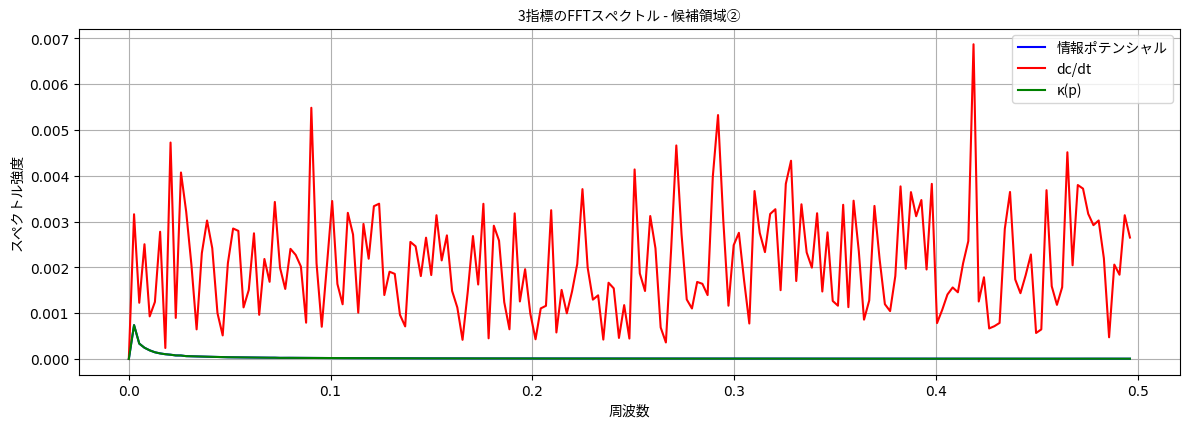
\includegraphics[width=\linewidth]{S1_fft_spectre_seq2.png}
        \caption{候補領域②のFFTスペクトル}
        \label{fig:supp_fft_region2}
    \end{subfigure}
    \vspace{1cm}
    \begin{subfigure}{0.48\linewidth}
        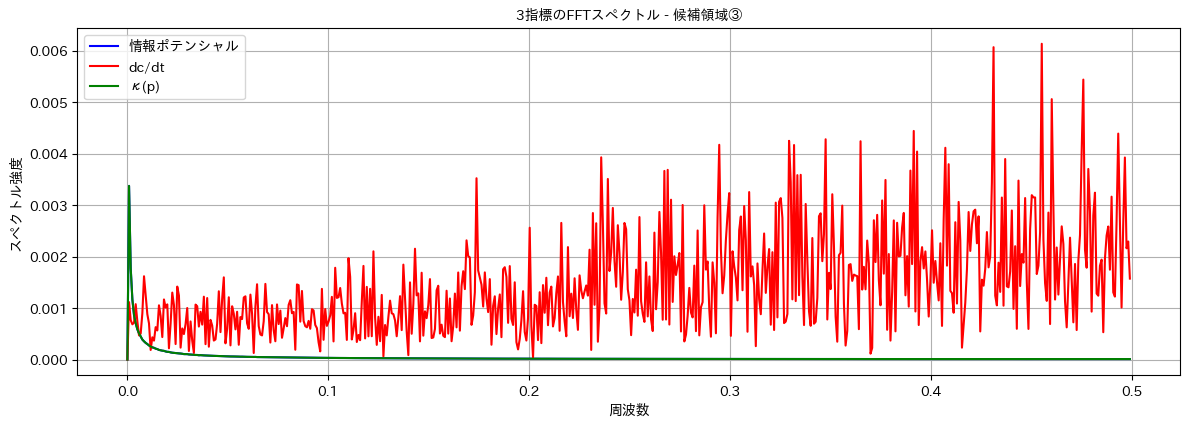
\includegraphics[width=\linewidth]{S1_fft_spectre_seq3.png}
        \caption{候補領域③のFFTスペクトル}
        \label{fig:supp_fft_region3}
    \end{subfigure}
    \hfill
    \begin{subfigure}{0.48\linewidth}
        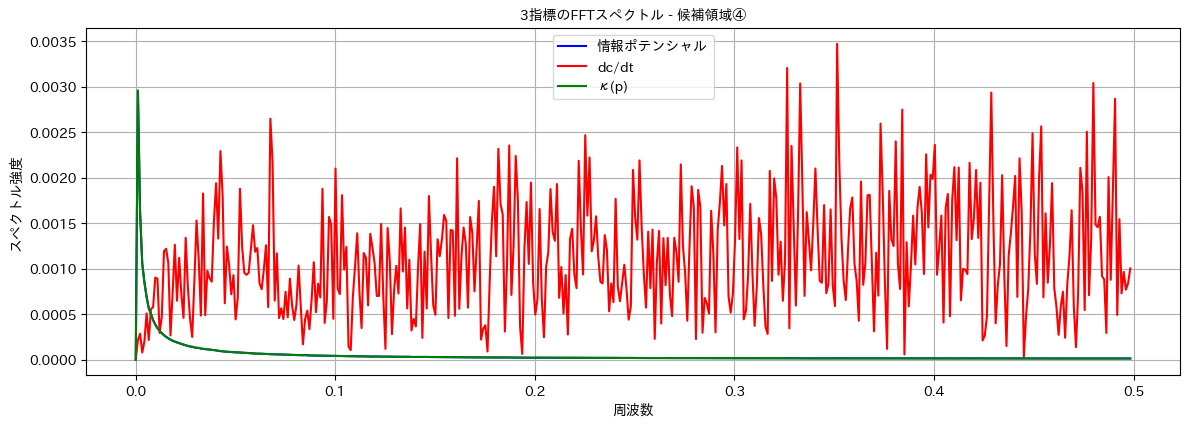
\includegraphics[width=\linewidth]{S1_fft_spectre_seq4.png}
        \caption{候補領域④のFFTスペクトル}
        \label{fig:supp_fft_region4}
    \end{subfigure}
    \caption{4つの異なる候補領域から抽出されたシーケンスにおける三指標のFFTスペクトル。}
    \label{fig:supp_fft_regions}
\end{figure}

\begin{table}[H]
    \centering
    \caption{各候補領域における三指標の卓越周波数と位相}
    \label{tab:supp_fft_peak_results}
    \begin{tabular}{@{}lccc@{}}
        \toprule
        \textbf{候補領域} & \textbf{指標} & \textbf{卓越周波数} & \textbf{位相 [deg]} \\
        \midrule
        \textbf{領域①} & 情報ポテンシャル & 0.0043 & 105.25 \\
                         & $\mathrm{d}c/\mathrm{d}t$ & 0.3621 & 106.76 \\
                         & $\kappa(p)$ & 0.0043 & 105.27 \\
        \midrule
        \textbf{領域②} & 情報ポテンシャル & 0.0026 & 92.35 \\
                         & $\mathrm{d}c/\mathrm{d}t$ & 0.4186 & 40.17 \\
                         & $\kappa(p)$ & 0.0026 & 92.35 \\
        \midrule
        \textbf{領域③} & 情報ポテンシャル & 0.0008 & 94.59 \\
                         & $\mathrm{d}c/\mathrm{d}t$ & 0.4553 & 41.32 \\
                         & $\kappa(p)$ & 0.0008 & 94.59 \\
        \midrule
        \textbf{領域④} & 情報ポテンシャル & 0.0011 & 98.46 \\
                         & $\mathrm{d}c/\mathrm{d}t$ & 0.3515 & -144.86 \\
                         & $\kappa(p)$ & 0.0011 & 98.46 \\
        \bottomrule
    \end{tabular}
\end{table}

表\ref{tab:supp_fft_peak_results}が明確に示すように、解析した4つの候補領域全てにおいて、情報ポテンシャルと$\kappa(p)$は共通の非常に低い卓越周波数を示し、かつその位相差はほぼゼロであった。これは、これら二指標が特定の低周波モードで強く結合し、同位相で振動するという動的同期が、局所的な現象ではなく、\#1点に関連する構造において普遍的に見られる特徴であることを強く示唆している。

\subsection*{S1.3. 階層的同期:$\mathrm{d}c/\mathrm{d}t$卓越周波数での応答}
\label{subsec:supp_hierarchical_sync}

§S1.2では、情報ポテンシャルと$\kappa(p)$が低周波で強く同期する一方で、$\mathrm{d}c/\mathrm{d}t$は異なる高周波で卓越するという、階層的なダイナミクスが示唆された。この階層性をさらに調査するため、$\mathrm{d}c/\mathrm{d}t$が卓越する周波数において、他の二指標がどのように応答するかを評価した。

候補領域①および②において、それぞれの$\mathrm{d}c/\mathrm{d}t$の卓越周波数をターゲット周波数とし、その周波数ビンにおける情報ポテンシャルと$\kappa(p)$のスペクトル強度および位相を再評価した。結果を図~\ref{fig:supp_fft_re_regions}および表~\ref{tab:supp_fft_re_results}に示す。

\begin{figure}[H]
    \centering
    \begin{subfigure}{0.48\linewidth}
        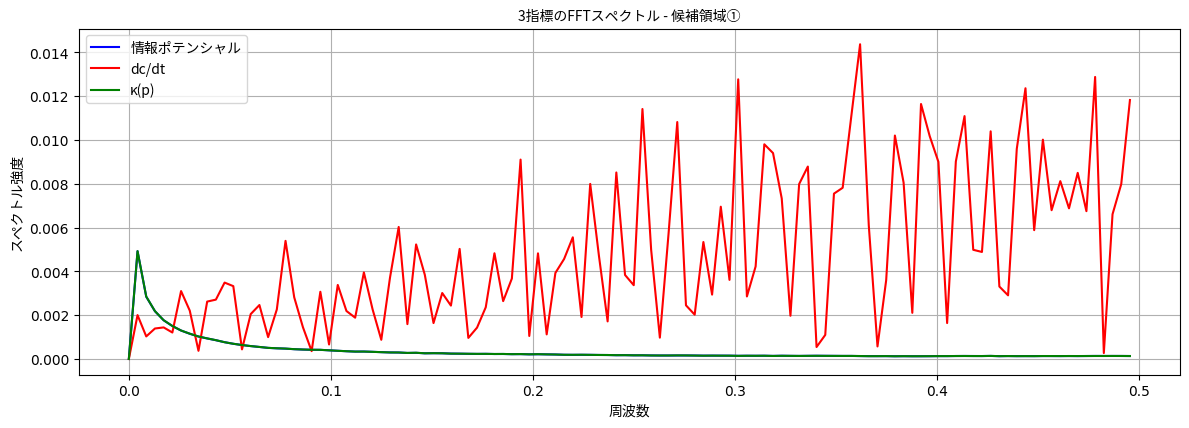
\includegraphics[width=\linewidth]{S1_fft_spectre_seq1.png}
        \caption{候補領域① ($\mathrm{d}c/\mathrm{d}t$卓越周波数ターゲット)}
        \label{fig:supp_fft_region1_re}
    \end{subfigure}
    \hfill
    \begin{subfigure}{0.48\linewidth}
        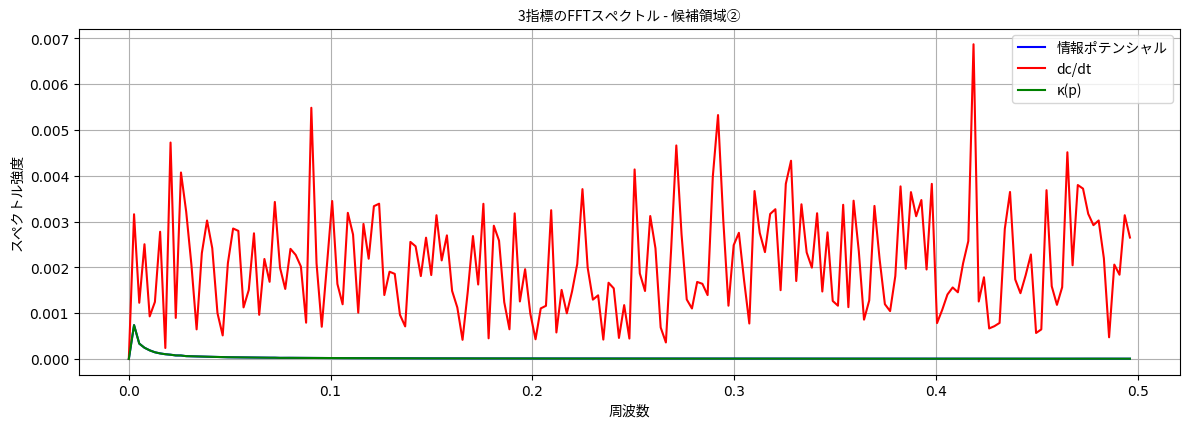
\includegraphics[width=\linewidth]{S1_fft_spectre_seq2.png}
        \caption{候補領域② ($\mathrm{d}c/\mathrm{d}t$卓越周波数ターゲット)}
        \label{fig:supp_fft_region2_re}
    \end{subfigure}
    \caption{候補領域①および②において、各領域の$\mathrm{d}c/\mathrm{d}t$の卓越周波数をターゲットとした三指標のFFTスペクトル。}
    \label{fig:supp_fft_re_regions}
\end{figure}

\begin{table}[H]
    \centering
    \caption{$\mathrm{d}c/\mathrm{d}t$の卓越周波数における各指標の応答}
    \label{tab:supp_fft_re_results}
    \begin{tabular}{@{}lccc@{}}
        \toprule
        \textbf{候補領域 @ Target Freq.} & \textbf{指標} & \textbf{強度 [a.u.]} & \textbf{位相 [deg]} \\
        \midrule
        \textbf{領域① @ 0.3621 Hz} & 情報ポテンシャル & $1.32 \times 10^{-4}$ & 154.32 \\
                         & $\mathrm{d}c/\mathrm{d}t$ & $1.44 \times 10^{-2}$ & 106.76 \\
                         & $\kappa(p)$ & $1.35 \times 10^{-4}$ & 154.32 \\
        \midrule
        \textbf{領域② @ 0.4186 Hz} & 情報ポテンシャル & $6.10 \times 10^{-6}$ & 166.76 \\
                         & $\mathrm{d}c/\mathrm{d}t$ & $6.87 \times 10^{-3}$ & 40.17 \\
                         & $\kappa(p)$ & $6.12 \times 10^{-6}$ & 166.51 \\
        \bottomrule
    \end{tabular}
\end{table}

表\ref{tab:supp_fft_re_results}が示すように、$\mathrm{d}c/\mathrm{d}t$が卓越する周波数において、情報ポテンシャルと$\kappa(p)$のスペクトル強度は$\mathrm{d}c/\mathrm{d}t$自身の強度と比較して2桁以上小さいものの、これら二つの指標は互いにほぼ完全に同位相で応答している(位相差は領域①で0.00°、領域②で0.25°)。

この結果は、系の基本的な状態を記述する情報ポテンシャルと$\kappa(p)$が、$\mathrm{d}c/\mathrm{d}t$によって引き起こされるより高周波な「揺さぶり」に対しても、足並みを揃えて応答することを示唆している。これは、低周波での強い同期と合わせて、「渦巻き位相」構造が持つ階層的で安定した動的特性を裏付けるものである。

\subsection{Ia型超新星データ単独でのパラメータ推定}
\label{subsec:supp_sne_only_fit}

DIRT Quadrupoleモデルのパラメータを制限する最初のステップとして、Ia型超新-星(Pantheon+)の全1701個のデータのみを用いたMCMC解析を実行した。

図\ref{fig:supp_mcmc_sne_only}に、このSNe単独解析で得られた各パラメータの事後確率分布を示す。また、得られた最も確からしい値(中央値)と1シグマ(68\%)信頼区間は以下の通りである。

\begin{figure}[H]
    \centering
    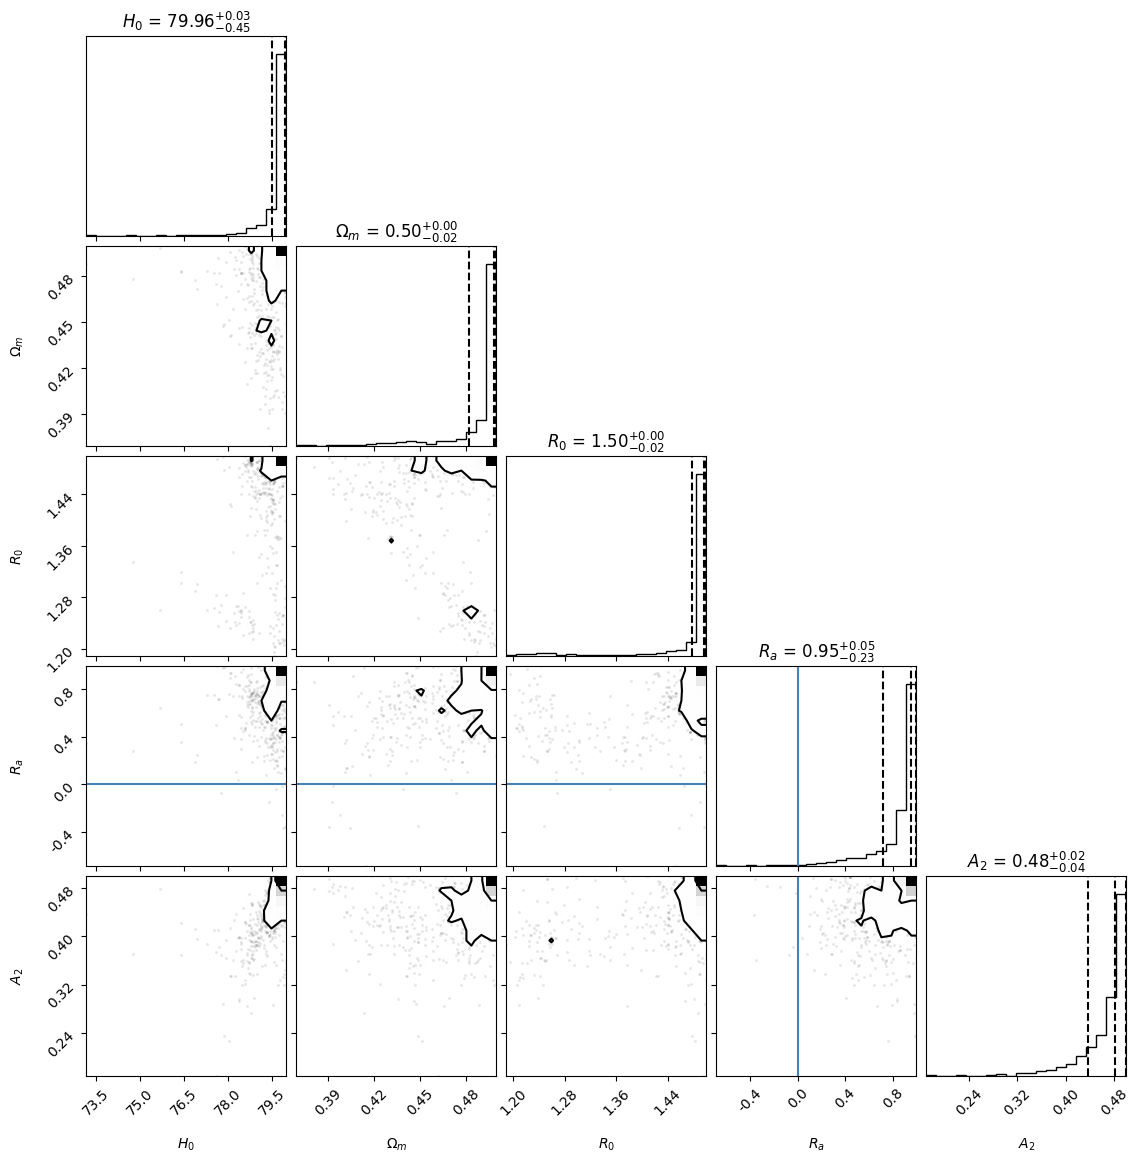
\includegraphics[width=\linewidth]{S2_MCMC_analysis_of_SNe_Ia_alone.png}
    \caption{SNe Iaデータ単独でのMCMC解析によって得られたパラメータのコーナープロット。}
    \label{fig:supp_mcmc_sne_only}
\end{figure}

\begin{itemize}
    \item $H_0 = 79.958 ^{+0.034} _{-0.448}$ km/s/Mpc
    \item $\Omega_m = 0.499 ^{+0.001} _{-0.017}$
    \item $R_0 = 1.497 ^{+0.003} _{-0.019}$
    \item $R_a = 0.951 ^{+0.047} _{-0.229}$
    \item $A_2 = 0.481 ^{+0.018} _{-0.044}$
\end{itemize}

この結果から、SNe Iaデータは、大きな非等方性の振幅($A_2 \approx 0.48$)を持つモデルを強く支持することがわかる。しかし、同時に$H_0$や$\Omega_m$といった宇宙論の基本パラメータが、標準$\Lambda$CDMモデルの推定値から大きく乖離しており、このモデルが他の観測と整合的であるかを検証する必要性が示唆された。これが、次節で述べるBAOデータとの比較、そして最終的な統合解析へと繋がる動機である。


\subsection{統合解析との比較とBAOデータの役割}
\label{subsec:supp_joint_comparison}

§\ref{subsec:supp_sne_only_fit}で示したSNe単独解析の結果は、大きな非等方性$A_2$を強く示唆した。本節では、この結果がBAOデータを加えた統合解析によってどのように変化したかを比較し、BAOデータが我々のモデルのパラメータ制限に果たした役割を考察する。

表\ref{tab:supp_param_comparison}に、SNe単独解析と、SNe+BAO統合解析(論文E本体 統合解析と非等方性の決定的証拠 参照)で得られた各パラメータの1シグマ信頼区間付きの最尤値を示す。

\begin{table}[H]
    \centering
    \caption{SNe単独解析とSNe+BAO統合解析のパラメータ推定値の比較}
    \label{tab:supp_param_comparison}
    \begin{tabular}{@{}lcc@{}}
        \toprule
        \textbf{パラメータ} & \textbf{SNe単独 (1701点)} & \textbf{SNe+BAO (統合解析)} \\
        \midrule
        $H_0$ [km/s/Mpc] & $79.958 ^{+0.034} _{-0.448}$ & $79.956 ^{+0.034} _{-0.148}$ \\
        $\Omega_m$ & $0.499 ^{+0.001} _{-0.017}$ & $0.499 ^{+0.001} _{-0.004}$ \\
        $R_0$ & $1.497 ^{+0.003} _{-0.019}$ & $1.198 ^{+0.002} _{-0.008}$ \\
        $R_a$ & $0.951 ^{+0.047} _{-0.229}$ & $0.981 ^{+0.016} _{-0.090}$ \\
        $A_2$ & $0.481 ^{+0.018} _{-0.044}$ & $0.488 ^{+0.011} _{-0.064}$ \\
        \bottomrule
    \end{tabular}
\end{table}

この比較から、以下の重要な点が明らかになる。

\begin{enumerate}
    \item \textbf{非等方性$A_2$の堅牢性}: これが最も重要な知見である。BAOという、宇宙の膨張史に対して非常に強力な制限を与えるデータを加えても、非等方性の振幅$A_2$の最尤値は$\approx 0.48$からほとんど変化せず、その信頼区間は依然として0を全く含まない。これは、SNe Iaデータが見出した非等方性のシグナルが、見かけの効果ではなく、BAOデータとも整合的な、極めて頑健な特徴であることを示している。
    \item \textbf{$R_0$の再調整}: 最も顕著な変化が見られたのは、$R_{lock}$の等方成分の現在値である$R_0$である。SNe単独では$\approx 1.5$という大きな値が好まれたのに対し、統合解析では$\approx 1.2$へと有意にシフトした。これは、BAOが要求する厳密な膨張史と、SNeが要求する非等方性を両立させるため、モデルが内部パラメータを「再調整」した結果と解釈できる。モデルは、$R_0$の値を下げることで、BAOデータへのフィットを改善しつつ、大きな$A_2$を維持するという、絶妙なバランス点を見つけ出したのである。
    \item \textbf{他パラメータの制限向上}: $H_0$, $\Omega_m$, $R_a$の各パラメータのエラーバーは、統合解析によって顕著に縮小した。これは、SNeとBAOという異なるプローブを組み合わせることが、パラメータ間の縮退を解消し、モデル全体の制限を大幅に向上させることを示している。
\end{enumerate}

総じて、この比較は、我々のDIRT Quadrupoleモデルの妥当性をさらに強固にするものである。BAOデータは非等方性の存在を否定するどころか、モデルの内部パラメータの値をより精密に決定するのに貢献し、SNeとBAOの両方を整合的に説明する非等方な宇宙像を、より高い信頼度で支持したのである。


\section*{S3. 実験的検証の提案(チェックリスト②)}
\label{sec:supp_experimental_proposal}

本研究の理論的・観測的成果、特に情報ロック係数$R_{lock}$の重要性を物理的に確立するためには、実験室スケールでの直接的な検証が不可欠である。本セクションでは、そのための具体的な光学卓上実験の計画を提案する。

\subsection*{S3.1. 実験コンセプトと目的}
\label{subsec:supp_exp_concept}

本実験の目的は、情報ロック係数 $R_{lock}$ を実験的に0から1の範囲で能動的に制御し、その変化に応じて物理系が示す「慣性」あるいは「有効質量 $m_{eff}$」の様相が、DIRT理論の予測に従って連続的に遷移するかを観測することである。この検証は、$R_{lock}$ の物理的実在性と、情報と質量・エネルギーの間の動的な連続性を実証する上で極めて重要となる。

\subsection*{S3.2. $R_{lock}$の定義と実験的制御}
\label{subsec:supp_exp_rlock_control}

本実験においては、論文Dで定義された情報ロック係数の基本式を用いる。
\begin{equation}
    R_{lock} = \frac{\tau_{det}}{\tau_{det}+\tau_{path}}\,(1-\beta_{scat})
    \label{eq:supp_rlock_experimental}
\end{equation}
ここで、当面は理想的な状況として散乱がない真空系($\beta_{scat} \approx 0$)を想定し、$R_{lock} \approx \tau_{det} / (\tau_{det}+\tau_{path})$ の制御を目指す。$\tau_{path}$(光子の伝搬時間)と$\tau_{det}$(検出・情報確定時間)は、それぞれ可変光ファイバ遅延線と後段の可変電子遅延モジュールを用いて、独立に制御する。この二段階スキャンにより、$R_{lock}$ の全動作範囲を実験的にカバーする。

\subsection*{S3.3. 提案実験系と測定量}
\label{subsec:supp_exp_setup_measurement}

提案する実験系の主要構成要素を図~\ref{fig:supp_exp_setup_schematic}の概念図に示す。
\begin{figure}[H]
    \centering
    \fbox{\parbox{0.8\linewidth}{\centering \vspace{5cm} (ここに実験セットアップの概念図を挿入予定:\\ 光源、可変光遅延線、MEMSミラー、干渉計、SNSPD、可変電子遅延などを含むブロック図) \vspace{5cm}}}
    \caption{提案される光学卓上実験の概念図(イメージ)。}
    \label{fig:supp_exp_setup_schematic}
\end{figure}

\begin{itemize}
    \item **光源**: 単一光子レベルに減衰されたピコ秒パルスレーザー(例:1550 nm帯)。
    \item **$R_{lock}$ 制御系**: 可変光ファイバ遅延線($\tau_{path}$制御用)および可変電子遅延モジュール($\tau_{det}$制御用)。
    \item **慣性プローブ**: 高Q値MEMSカンチレバーまたは薄膜ミラー。光パルスからの運動量移行(光圧)を受けて微小変位する。
    \item **変位検出系**: MEMSミラーの微小変位を高感度で読み出すための光干渉計。
    \item **光子検出器**: SNSPD。光子の到達時刻を高精度で記録、あるいは実験全体のトリガー/同期に使用。
\end{itemize}

測定する主要な物理量は、MEMSミラーが受ける光圧による運動量移行である。各$R_{lock}$値において、一定エネルギーの光パルス列をMEMSミラーに入射し、その変位応答を精密に測定する。測定された力積(運動量 $p$)や系の応答特性を、「有効質量 $m_{eff}$」あるいは「慣性の指標」の代理変数と定義し、横軸に$R_{lock}$、縦軸に$m_{eff}$をプロットすることで、$m_{eff}(R_{lock})$ の連続遷移曲線の作成を目指す。

DIRT理論は、$R_{lock} \to 0$(エネルギー優勢極限)で $m_{eff} \to 0$、$R_{lock} \to 1$(質量優勢極限)で $m_{eff}$ がある有限値に飽和する、という連続的な遷移を予測する。この実験的曲線と理論予測を比較することが、本実験の最終目標である。

\end{document}